%!TEX root = ../thesis.tex

%%%%%%%%%%%%%%%%%%%%%%%%%%%%%%%%%%%%%%%%%%%%%%%%%%%%%%
%%%%%%%%%%%%%%%%%%%%%%%%%%%%%%%%%%%%%%%%%%%%%%%%%%%%%%
\subsection{Trabalhos relacionados}
\begin{frame}{Trabalhos relacionados}
	Plataformas de desenvolvimento de MABS
	\begin{itemize}
		\item Domínio específico (p.e. MASeRaTi, MATSim, SUMO)
		\item Propósito geral (p.e. Repast, NetLogo, GALATEA, PlaSMA)
	\end{itemize}

	Foco em integração de simulação no JADE (p.e. MISIA, JRep, PlaSMA)
\end{frame}

\begin{frame}{MISIA}
	BISITE, Universidad de Salamanca (\url{bisite.usal.es})

	\begin{figure}
		\centering
		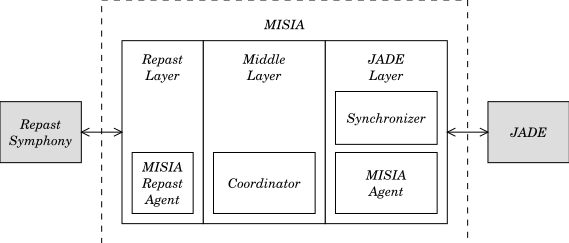
\includegraphics[height=4cm]{figures/MISIA.pdf}
	\end{figure}
\end{frame}

\begin{frame}{JRep}
	Niedersächsische Technische Hochschule (\url{www.nth-online.org})

	\begin{figure}
		\centering
		\includegraphics[height=4cm]{figures/jrep.pdf}
	\end{figure}
\end{frame}

\begin{frame}{PlaSMA}
	TZI, Universität Bremen (\url{www.tzi.de})

	\begin{figure}
		\centering
		\includegraphics[height=4cm]{figures/PlaSMA.pdf}
	\end{figure}
\end{frame}

\begin{frame}{Comparação}
	\begin{itemize}
		\item JRep, MISIA não são projetos ativos
		\item Os três exemplos dependem da plataforma JADE durante a simulação
	\end{itemize}
\end{frame}

%%%%%%%%%%%%%%%%%%%%%%%%%%%%%%%%%%%%%%%%%%%%%%%%%%%%%%
%%%%%%%%%%%%%%%%%%%%%%%%%%%%%%%%%%%%%%%%%%%%%%%%%%%%%%
\subsection{JADE e Repast}

\begin{frame}{JADE}
	\begin{table}[h]
		\label{tab:jadevsrep}
		\tiny
		\begin{center}
			\begin{tabular}{l|cc}
			\hline

			\hline
			\textbf{} & \textbf{JADE} & \textbf{Repast} \\ %& \textbf{Cougaar} \\
			\hline
				Comunicação & FIPA ACL &  Acesso direto  \\ %& Serialized Object \\
							  &			 &  Partilha de recursos \\
			\hline
				Distribuído & Sim & Não \\ 
			\hline
				Simulação & Não & Sim \\ 
			\hline
				Escalabilidade & Limitada & Elevada \\ 
			\hline
				Ontologias & Sim & Não \\
			\hline
				Execução de & Behaviours 	& Escalonamento  	\\ %&  \\
				Agentes		& Multi thread 	& Single thread 	\\ %&  \\
							& Eventos   	& Ticks		 	   	\\ %&  \\
							& Assíncrona 	& Síncrona 		   	\\ %&  \\
			\hline
				Código Livre & Sim & Sim \\ 
			\hline
				Linguagem & Java & Java \\ 
			\hline
			\end{tabular}
		\end{center}
		\caption{Comparação entre JADE e Repast.}
	\end{table}
\end{frame}

%%%%%%%%%%%%%%%%%%%%%%%%%%%%%%%%%%%%%%%%%%%%%%%%%%%%%%
%%%%%%%%%%%%%%%%%%%%%%%%%%%%%%%%%%%%%%%%%%%%%%%%%%%%%%
\subsection{Especificações FIPA no JADE}
\begin{frame}{Especificações FIPA no JADE}
	Três conceitos principais:
		\begin{itemize}
			\item Gestão de Agentes (DF, AMS, AID)
			\item Serviço de Mensagens (MTS, ACL Message)
			\item Protocolos de interação (FIPA Request, FIPA Contract Net)
		\end{itemize}
		
\end{frame}


